\documentclass[../fapesp0]{subfiles}

\begin{document}

\chapter{Realizações no período}

No primeiro semestre do mestrado, foram cursadas\footnote{Meu diploma de graduação foi emitido pela Unicamp três dias após o início das aulas da USP. Por razões burocráticas que não puderam ser contornadas, não foi possível realizar a matrícula em nenhuma disciplina no primeiro semestre, então as mesmas foram assistidas como ouvinte e estão sendo ``aproveitadas'' no primeiro semestre de 2024.} as disciplinas de Medida e Integração, Topologia Algébrica e Geometria Riemanniana. Em relação à pesquisa, participei de seminários do grupo de dinâmica e realizei leitura prévia de alguns materiais importantes para o projeto.
No segundo semestre de 2023, cursei as disciplinas de Teoria Ergódica, Teoria Geométrica de Medidas e Preparação Pedagógica e iniciamos reuniões semanais para discussão do artigo \citetitle{bonifantSchwarzianDerivativesCylinder2008}.

De janeiro a fevereiro de 2024, participei de uma escola de verão sobre dinâmica parcialmente hiperbólica e cursei Análise Funcional no programa de verão do IMPA. Em seguida, começamos a aprofundar sobre o fenômeno de comportamento histórico, usando como base o caso da Schwarziana nula e o artigo \cite{crovisierEmpiricalMeasuresPartially2020}.

\section{Medidas empíricas}

O conceito principal do projeto é o de medida empírica. As medidas empíricas associam a cada ponto do espaço uma sequência de medidas que capturam a média do que foi observado ao longo de uma órbita até certo tempo.

Fixemos um espaço métrico compacto \(X\) com a \(\sigma\)-álgebra de Borel, e \(f \colon X \to X\) uma transformação mensurável. 
\begin{definition}
  Dado \(x \in X\), a \emph{medida empírica} no tempo \(n\) é a medida
  \begin{equation*}
    e_n(x) = \frac{1}{n} \sum_{k = 0}^{n - 1}\delta_{f^k(x)}.
  \end{equation*}
\end{definition}

\begin{definition}
  Seja \((\mu_n)_{n \in \NN} \subseteq \Meas[1]{X}\) uma sequência de medidas. Dizemos que \((\mu_n)_n\) \emph{converge fracamente} a \(\mu\), ou \(\mu_n \weakto \mu\), se a sequência converge na topologia fraca-estrela de \(\Meas[1]{X} \subseteq \Cs{X}^*\). Isso significa que para toda \(\varphi \in \Cs{X}\), vale \(\int \varphi \;d\mu_n \to \int \varphi \;d\mu\).
\end{definition}

\begin{proposition}[Portmanteau]\label{prop:portmanteau}
  São equivalentes:
  \begin{enumerate}[a), left=0pt, topsep=3pt]
    \item \(\mu_n \weakto \mu\);
    \item \(\lim_{n \to \infty} \mu_n(\phi) = \mu(\phi)\) para toda função Lipschitz \(\phi\);
    \item \(\liminf_{n \to \infty} \mu_n(U) \geq \mu(U)\) para todo aberto \(U \subseteq X\);
    \item \(\limsup_{n \to \infty} \mu_n(F) \leq \mu(F)\) para todo fechado \(F \subseteq X\);
    \item \(\lim_{n \to \infty} \mu_n(A) \leq \mu(A)\) para todo conjunto de continuidade \(A\) da medida \(\mu\), isto é, tal que \(\mu(\partial A) = 0\).
  \end{enumerate}
\end{proposition}

\begin{definition}
  Seja \(\mu \in \Meas[1]{X}\) uma medida invariante por \(f\). A \emph{bacia} da medida \(\mu\) é o conjunto
  \begin{equation*}
    \mathcal{B}(\mu) = \set{ x \in X : e_n(x) \weakto \mu }.
  \end{equation*}
\end{definition}

\begin{lemma}
  Para todo \(\mu \in \Meas[1]{X}\), \(\mathcal{B}(\mu)\) é um conjunto estritamente invariante.
\end{lemma}

\begin{lemma}\label{lem:basins-disjoint}
  Se \(\mu, \nu \in \Meas[1]{X}\) são medidas invariantes distintas, então \(\mathcal{B}(\mu) \cap \mathcal{B}(\nu) = \varnothing\).
\end{lemma}

\begin{corollary}
  Se \(\mu \in \Meas[1]{X}\) é uma medida invariante, então \(\mu(\mathcal{B}(\mu)) = 1\) se \(\mu\) for ergódica e \(\mu(\mathcal{B}(\mu)) = 0\) caso contrário.
\end{corollary}

\begin{proof}
  Se \(\mu\) for ergódica, por Birkhoff e pelo fato de \(\Cs{X}\) ser separável, existe um conjunto de medida \(\mu\) total em que \(e_n(x) \weakto \mu\).

  Caso contrário, seja \(\{ \mu_x \}_{x \in X}\) a decomposição ergódica de \(\mu\). Como \(\mu_x \neq \mu\) para quase todo \(x\), pelo lema e caso anterior \(\mu_x(\mathcal{B}(\mu)) = 0\), portanto
  \begin{equation*}
    \mu(\mathcal{B}(\mu)) = \int \mu_x(\mathcal{B}(\mu)) \;d\mu(x) = 0.
  \end{equation*}
  
\end{proof}

\section{O exemplo de Bonifant-Milnor}
Em~\cite{bonifantSchwarzianDerivativesCylinder2008}, os autores construíram uma família de difeomorfismos do tipo \textit{skew product} cujas propriedades dinâmicas variam de acordo com a derivada Schwarziana dos mapas nas fibras. Dependendo do sinal dessa derivada, a família possui bacias entrelaçadas, uma medida física cuja bacia tem medida de Lebesgue completa, ou comportamento histórico em quase todo ponto. Durante o primeiro ano, procuramos entender bem essa família de exemplos e responder algumas questões postas no artigo.


\subsection{Razão cruzada e a derivada Schwarziana}

Suponha que começamos com um corpo \(\mathbb{K}\) e, não estando suficientemente contentes com o fato de não podermos dividir por zero, decidimos adicionar um ponto no infinito; isso nos dá a \textit{reta projetiva} \(P^1(\mathbb{K}) = \mathbb{K} \sqcup \{ \infty \}\), cujas operações aritiméticas são as mesmas de \(\mathbb{K}\) exceto pelas regras adicionais que
\(\frac{1}{0} = \infty\), \(\frac{1}{\infty} = 0\), \(x \cdot \infty = \infty\) se \(x \neq 0\) e \(x + \infty = \infty\) se \(x \neq \infty\).
Não é possível ficarmos totalmente contentes sem introduzir regras inconsistentes, e por isso as operações são parciais --- não podemos multiplicar \(\infty \cdot 0\) ou somar \(\infty + \infty\).

Nosso novo espaço \(P^1(\mathbb{K})\) tem uma propriedade interessante: dado \(z \in P^1(\mathbb{K})\), temos três tipos de operações que podemos aplicar em \(z\): translações \(z \mapsto z + x\), onde \(x \in \mathbb{K}\), homotetias \(z \mapsto xz\) para \(x \in \mathbb{K} \setminus \{ 0 \}\), e a inversa \(z \mapsto 1/z\), que antes não era definida se \(z = 0\), mas que agora faz sentido para todo \(z\). Essas três famílias de ações, que são invertíveis, geram o \textit{grupo de homografias} com coeficientes em \(\mathbb{K}\).

Uma segunda maneira de construir \(P^1(\mathbb{K})\), e que deixa bem mais claro o papel do grupo de homografias como grupo de simetrias deste espaço, é pensar no espaço de ``frações formais'', ou seja, nos pares de números \((x,y)\), onde \(x, y \in \mathbb{K}\) não são ambos zero, onde identificamos ``frações equivalentes'', no sentido de que \((\lambda x, \lambda y) \sim (x, y)\) para todo \(\lambda \in \mathbb{K} \setminus \{ 0 \}\). O quociente por essa relação de equivalência nos dá \(P^1(\mathbb{K})\) como o espaço das retas passando pela origem do espaço vetorial \(\mathbb{K}^2\), e as operações são como as operações de frações: \((x,y) + (z,w) = (wx + yz, yw)\), \((x,y) \cdot (z,w) = (xz, yw)\) e \((x,y)^{-1} = (y,x)\). Apesar de aparentemente mais complicada, o interessante dessa construção é que fica claro como o grupo de simetrias do espaço \(\mathbb{K}^2\), o grupo linear \(\GL_2(\mathbb{K})\), naturalmente induz um grupo de simetrias no quociente, o grupo projetivo \(\PGL_2(\mathbb{K})\), que é precisamente o grupo de homografias.

O interessante desse grupo é que ele é o quociente de \(\GL_2(\mathbb{K})\) por um subgrupo de dimensão \(1\), logo tem dimensão \(3\). Além do mais, ele é \(3\)-transitivo: dadas duas triplas de pontos distintos de \(P^1(\mathbb{K})\), existe um elemento \(g \in \PGL_2(\mathbb{K})\) que leva a primeira tripla na segunda. Mas não só isso, \(P^1(\mathbb{K})\) tem três pontos especiais: \(0\), \(1\) e \(\infty\). Assim, dados \(x_1,x_2, x_3 \in P^1(\mathbb{K})\) distintos, podemos nos perguntar qual o \(g \in \PGL_2(\mathbb{K})\) tal que \(g(x_1) = \infty\), \(g(x_2) = 0\) e \(g(x_3) = 1\). Com algumas contas, chegamos em 
\begin{equation*}
  g(z) = \frac{(x_2 - z)(x_3 - x_1)}{(x_1 - z)(x_3 - x_2)}
\end{equation*}
A \emph{razão cruzada} de quatro pontos \(x_{0},x_1,x_2,x_3\) é o valor de \(g(x_0)\) para o elemento \(g\) do grupo de homografias que envia \(x_1 \mapsto \infty\), \(x_2 \mapsto 0\) e \(x_3 \mapsto 1\).
\begin{definition}[Razão cruzada]
  \begin{equation*}
    \rho(x_0,x_1,x_2,x_3) = \frac{(x_2 - x_0)(x_3 - x_1)}{(x_1 - x_0)(x_3 - x_2)}
  \end{equation*}
\end{definition}

\NewObject\IFunOp\SchD{\mathcal{S}}
\begin{definition}

  Seja \(\f \colon I \to I'\) um difeomorfismo \(\Cs[d = 3]\) entre dois intervalos da reta.
  A \emph{derivada Schwarziana} de \(\f\) é a função
  \begin{equation*}
    \SchD\f = \frac{\f[der = 3]}{\f[der = 1]} - \frac{3}{2}\rpar*{\frac{\f[der = 2]}{\f[der = 1]}}^2.
  \end{equation*}
\end{definition}
Denotaremos \(\SchD f \prec 0\) caso exista um aberto denso \(U \subseteq I\) tal que \(\SchD f(y) < 0\) para todo \(y \in U\). Analogamente, denotaremos \(\SchD f \succ 0\) caso exista \(U \subseteq I\) aberto e denso tal que \(\SchD f(y) > 0\) para todo \(y \in U\).

\begin{proposition}\label{prop:schwarzian}
  A derivada Schwarziana tem as seguintes propriedades:
  \begin{enumerate}
    \item Se \(\mathcal{S}f\) e \(\mathcal{S}g\) possuem o mesmo sinal, então \(\mathcal{S}(g \circ f)\) tem o mesmo sinal.
    \item Se \(\mathcal{S}f \prec 0\), então \(\mathcal{S}f^{-1} \succ 0\). 
    \item \(\SchD f \prec 0\) se, e somente se, \(\varphi(y) = 1/ \sqrt{\lvert f'(y) \rvert}\) é estritamente convexa.
    \item \(\SchD f \equiv 0\) se, e somente se, \(f\) é uma transformação linear fracionária.
  \end{enumerate}
\end{proposition}

\begin{lemma}\label{lem:sch-cross-increase}
  Se \(f \colon I \to I'\) é \(C^3\), então \(\SchD f \prec 0\) se, e somente se, \(f\) aumenta cross-ratios, no sentido que \(\rho(f(y_{1}),f(y_2),f(y_3),f(y_4)) > \rho(y_{1},y_2,y_3,y_4)\) para todos \(y_1 < y_2 < y_3 < y_{4}\).
\end{lemma}

\begin{lemma}\label{lem:bound-deriv-schwarz}
  Se \(f \colon I \to I\) preserva a orientação e \(\SchD f \prec 0\), então \(f'(0)f'(1) < 1\).
\end{lemma}

Note que pela \cref{prop:schwarzian}, valem resultados análogos as últimos três lemas se \(\SchD f \succ 0\). Por exemplo, se \(\SchD f \succ 0\) então \(f\) diminui razões cruzadas e \(f'(0)f'(1) > 1\). 

\subsection{Produtos tortos}
Chamamos um mapa \(F \colon X \times Y \to X \times Y\) de \emph{produto torto} (ou \textit{skew product}) se ele é da forma \(F(x,y) = (g(x), f_x(y))\). Estamos interessados no caso em que \(X\) é um espaço métrico compacto (com a \(\sigma\)-álgebra de Borel), \(g \colon X \to X\) é um mapa contínuo que preserva uma medida ergódica \(\mu \in \Meas{X}\), \(Y = I\) é o intervalo \([0,1]\) e \(f_x \colon I \to I\) são difeomorfismos \(\Cs^3\) que preservam a orientação. Veremos como, a depender da derivada Schwarziana dos mapas \(f_x\), observamos diferentes comportamentos da dinâmica em relação às medidas invariantes \(\nu_0 = \mu \otimes \delta_0\) e \(\nu_1 = \mu \otimes \delta_1\). Note que para \(i \in \{ 0,1 \}\), \(\supp \nu_i = \mathcal{A}_i\), onde \(\mathcal{A}_i = X \times \{ i \}\) são os bordos do ``cilindro'' \(X \times Y\).
Seja também \(\mathcal{B}_i = \mathcal{B}(\nu_i)\) as bacias das respectivas medidas.

Para simplificar a notação, vamos denotar por \(f_x^{n}(y)\) a segunda coordenada de \(F^n(x,y)\), ou seja, \(f_x^{n} = f_{g^{n - 1}(x)} \circ \cdots \circ f_x\).

\begin{lemma}\label{lem:basin-segment}
  Se \((x, y_1) \in \mathcal{B}_0\), então \((x,y_2) \in \mathcal{B}_0\) para todo \(y_2 \leq y_1\). Analogamente, se \((x, y_1) \in \mathcal{B}_1\), então \((x,y_2) \in \mathcal{B}_0\) para todo \(y_2 \geq y_1\).
\end{lemma}

\begin{proof}
  Vamos demonstrar o caso \(i = 0\). Seja \((x,y_1) \in \mathcal{B}_0\) e \(y_2 \leq y_1\). Se \(\varphi \in \Cs{X \times I}\), e \(\varepsilon > 0\), pela continuidade uniforme de \(\varphi\), existe \(\delta > 0\) tal que \(y < \delta\) implica em \(\lvert \varphi(x,0) - \varphi(x,y) \rvert < \varepsilon\) para todo \(x \in X\). Como \(U = X \times \interval[open right]{0}{\delta}\) é um conjunto de continuidade para \(\nu_0\) e \(e_n(x,y_2) \to \nu_0\), por \nameref{prop:portmanteau}
    \newcommand{\timeinU}{\frac{1}{n}\# \set{ 0 \leq i < n \where f_x^n(y_2) < \delta }}
    \[\lim_{n \to \infty} e_n(x,y_2)(U) = \nu_0(U) = 1.\]
    Defina \(\tau_n = e_n(x,y_2)(U) = \timeinU\).
    Note que se \(f_x^n(y_2) < \delta\), então \(f_x^n(y_1) < \delta\) já que os difeomorfismos preservam orientação. Assim,
    \begin{align*}
      \lvert e_n(x,y_1)(\varphi) - e_n(x,y_2)(\varphi) \rvert
      &\leq \frac{1}{n}\sum_{i = 0}^{n - 1}\abs*{\varphi(g^n(x),f_x^{n}(y_1)) - \varphi(g^n(x),f_x^{n}(y_2))}\\
      &\leq \varepsilon \tau_n + 2 \lVert \varphi \rVert_{\infty} (1 - \tau_n).
    \end{align*}
    Como \(\tau_n \to 1\), existe \(N\) tal que \(n \geq N\) implica que o lado direito é menor que \(2 \varepsilon\), portanto ambas as integrais convergem para \(\nu_0(\varphi)\).
\end{proof}

\subsection{Bacias entrelaçadas}

\begin{wrapstuff}[type=figure,width=.4\textwidth,height=5cm]
  \centering
  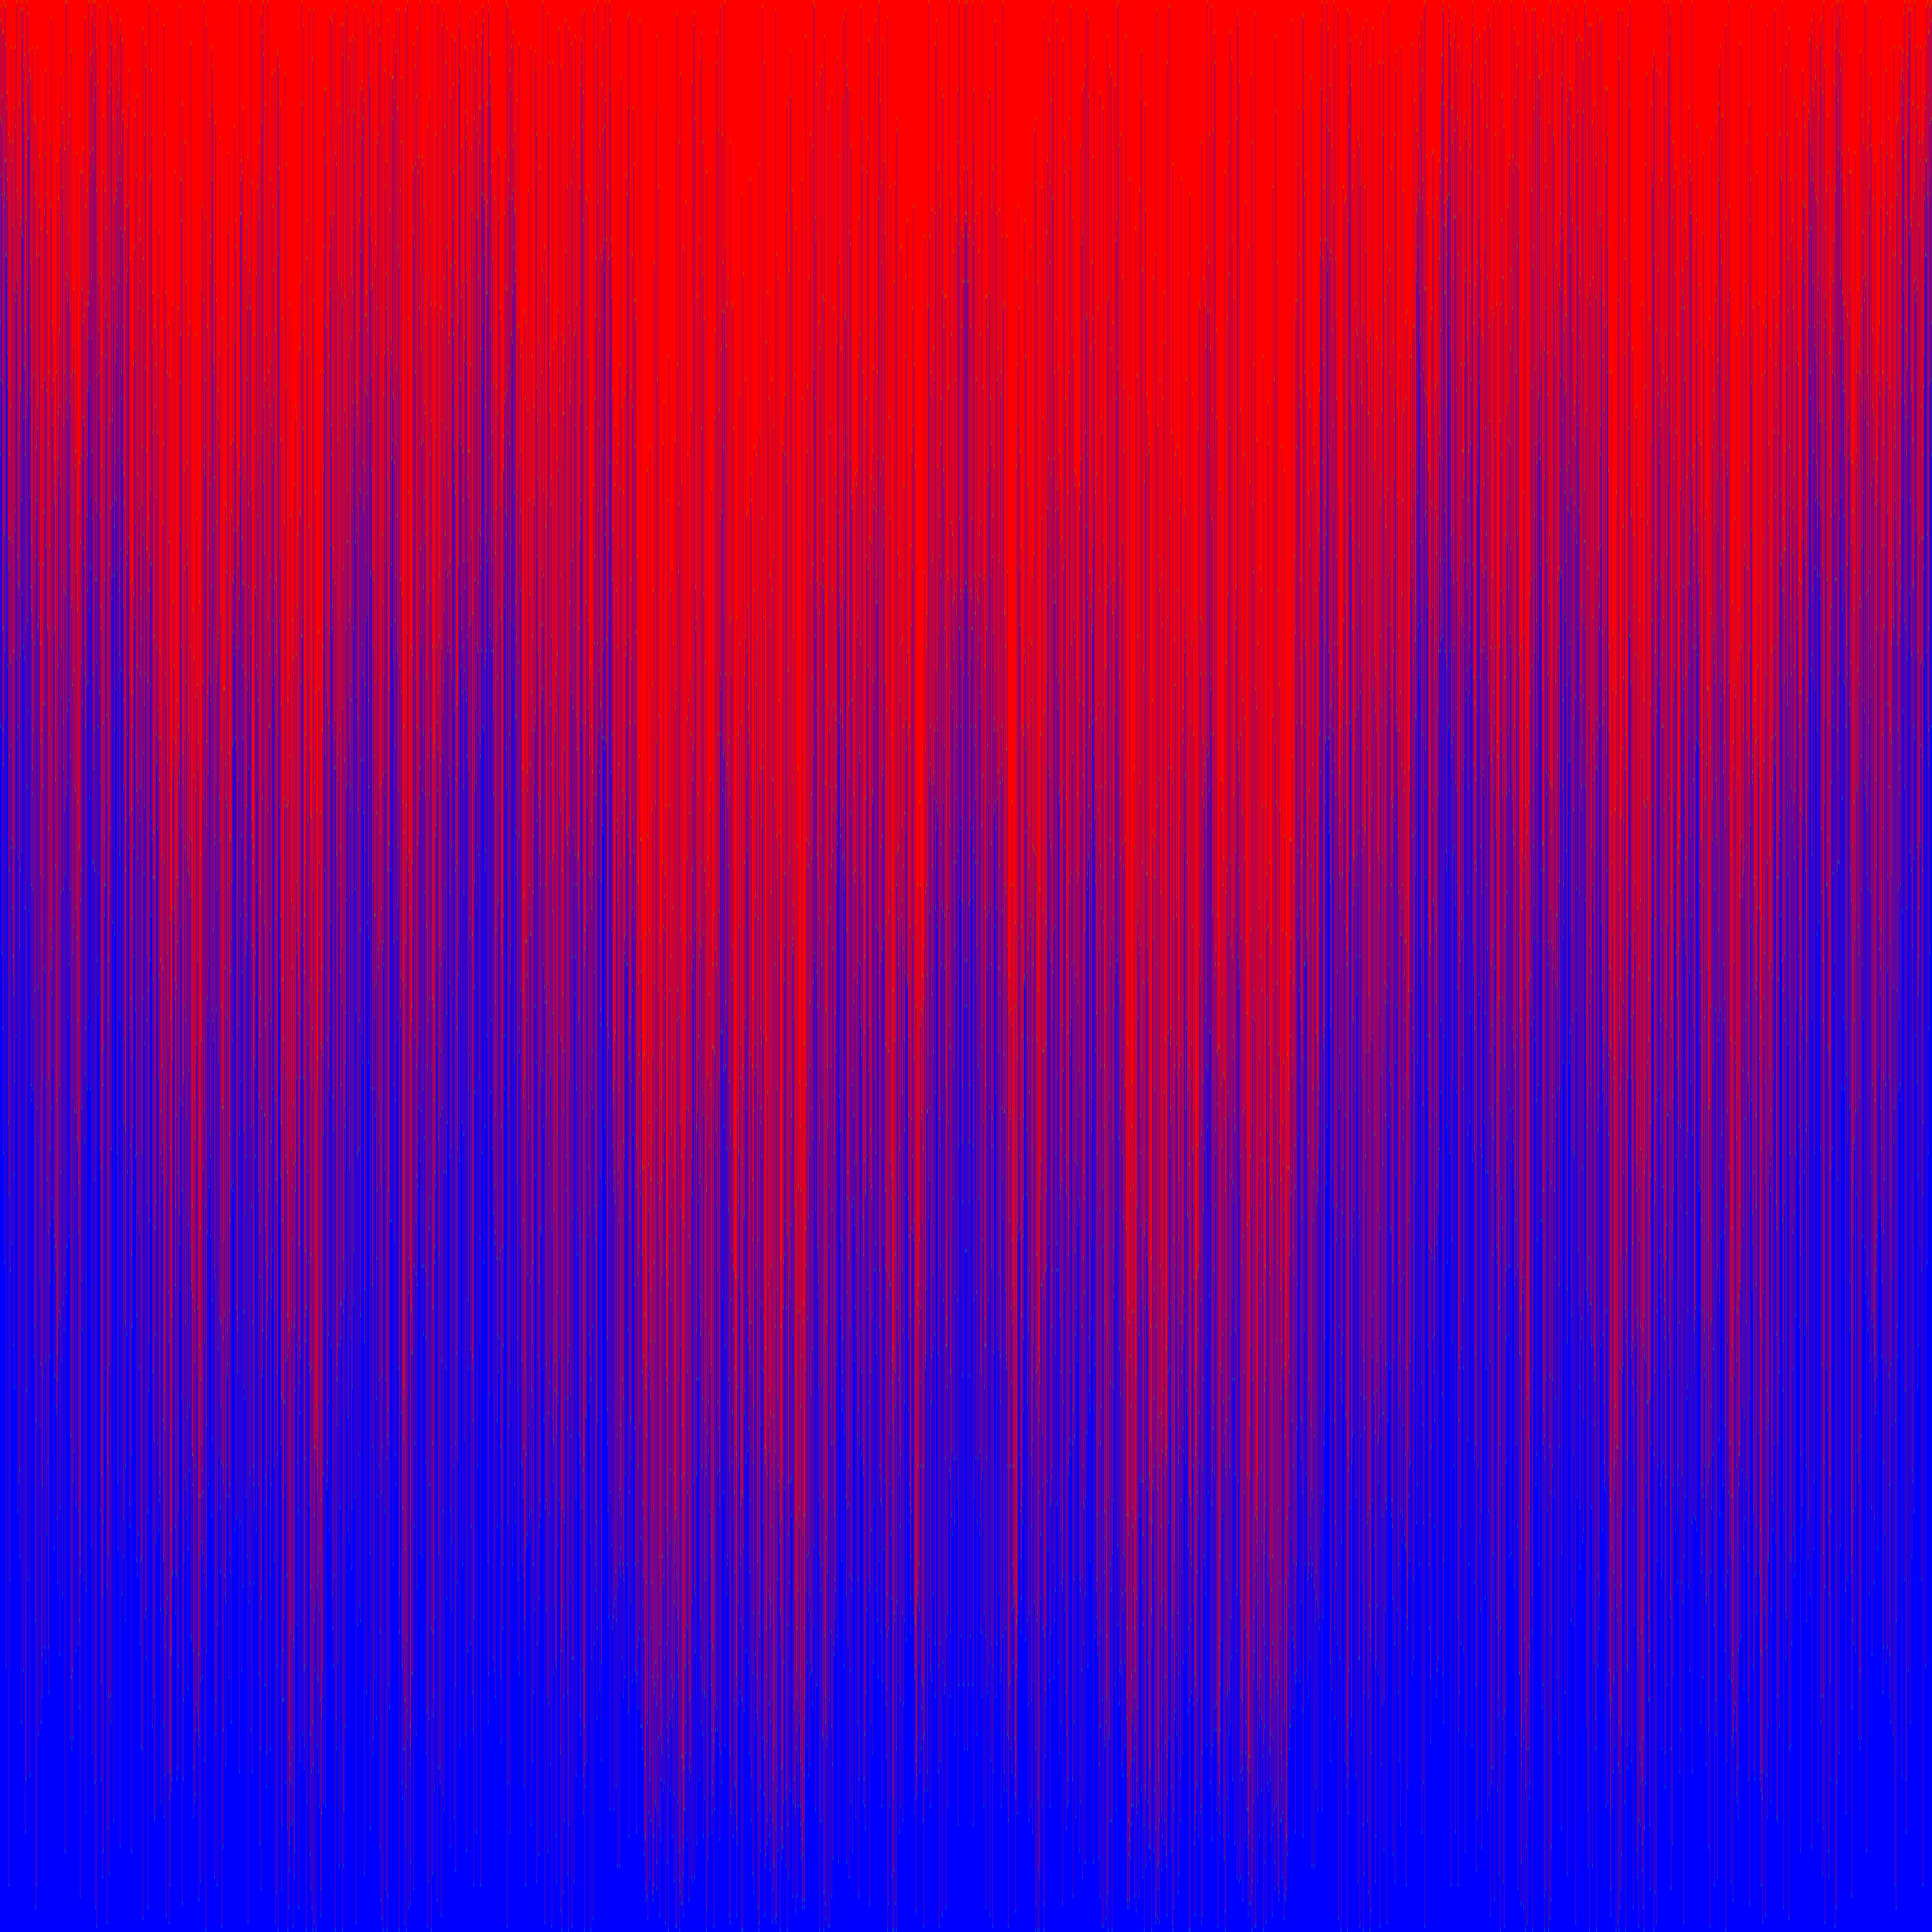
\includegraphics[width=0.8\linewidth]{../figures/intermingled}
  \caption{Bacias do \cref{ex:intermingled}.}
\end{wrapstuff}

Apenas nesta seção, fixaremos \(X = S^1\), \(\mu = \Leb\) e \(g \colon S^1 \to S^1\) o mapa \(g(x) = kx\). Além disso, pedimos que a seguinte hipótese seja satisfeita.

\begin{hypothesis}[Elevadores]\label{hip:elevators}
  Existem pontos fixos \(x^-\) e \(x^+\) em \(S^1\) tais que para todo \(y \in (0,1)\), \(f_{x}(y) < y\) para \(x\) em uma vizinhança de \(x^-\) e \(f_x(y) > y\) para \(x\) em uma vizinhança de \(x^+\).
\end{hypothesis}

\begin{definition}
  Dizemos que dois subconjuntos mensuráveis \(A, B\) são \textit{entrelaçados} em relação a uma medida \(\nu\) se para todo aberto \(U\), \(\nu(A \cap U)\) e \(\nu(B \cap U)\) são estritamente positivos.
\end{definition}

\begin{theorem}
  Suponha que vale a \cref{hip:elevators} e ambas as bacias têm medida positiva. Então as bacias \(\mathcal{B}_0\) e \(\mathcal{B}_1\) são entrelaçadas para a medida de Lebesgue no cilindro.
\end{theorem}

\begin{proof}
  Por definição, as bacias são conjuntos estritamente invariantes. Se definimos as medidas \(\mu_i(A) = \Leb(A \cap \mathcal{B}_i)\), então as bacias são entrelaçadas se, e somente se, \(\supp \mu_i = X \times I\) para ambos \(i = 0,1\). Mostraremos que este é o caso para \(\supp \mu_0\), já que para \(i = 1\) a demonstração é análoga.

  \begin{claim}
    O suporte \(\supp \mu_0\) é tal que \(F ^{-1}(\supp \mu_0) \subseteq \supp \mu_0\).
  \end{claim}
  De fato, se \(p \in F^{-1}(\supp \mu_0)\) e \(U\) é uma vizinhança de \(p\), então por \(F\) ser um mapa aberto, \(F(U)\) é uma vizinhança de \(F(p) \in \supp \mu_0\), logo \(\mu_0(F(U)) > 0\). Como \(F\) é Lipschitz, caso \(\mu_0(U)\) fosse \(0\) então \(\mu_0(F(U)) =\Leb(F(U) \cap \mathcal{B}_0) = \Leb(F(U \cap \mathcal{B}_0)) = 0\), o que não acontece, logo \(\mu_0(U) > 0\).

  \begin{claim}
    Existe um ponto \((x_0,y_0) \in \supp \mu_0 \setminus X \times \{ 0 \}\).
  \end{claim}
  De fato, \(\mu_0(\supp \mu_0) \geq \Leb(\mathcal{B}_0) > 0\), portanto \(\mu_0(\supp \mu_0 \setminus X \times \{ 0 \}) > 0\) e o conjunto não pode ser vazio.

  \begin{claim}
    A extremidade \(\mathcal{A}_1\) do cilindro está contida em \(\supp \mu_0\).
  \end{claim}
  Indutivamente, podemos construir uma órbita inversa \(\cdots \mapsto x_{-2} \mapsto x_{-1} \mapsto x_0\) de \(g\) de tal forma que \(x_{ - n - 1} \in g^{-1}(\{ x_{-n} \})\) seja a pré-imagem mais próxima de \(x_-\). Como \(x_-\) é um ponto fixo repulsor, a construção implica que \(x_{-n} \to x_-\), logo pela \cref{hip:elevators}  para todo \(y \in (0,1)\) existe \(n_0\) tal que \(n \geq n_0\) implica \(f_{x_{-n}}^{-1}(y_0) > y\). Em particular,
  \[y_{ - n} = f_{x_{-n}}^{-1} \circ \cdots \circ f_{x_{-1}}^{-1}(y_0)\]
  é tal que \(y_{ - n} \to 1\). Como \(\supp \mu_0\) é fechado e \((x_{ - n},y_{ - n}) \in F^{-n}(\supp \mu_0)\), concluímos que \((x_-, 1) \in \supp \mu_0\). Agora, note que \(E = \bigcup_{n = 0}^{\infty}g ^{-1}(\{ x_- \})\) é denso em \(X\) e \(1\) é ponto fixo das \(f_x\). Assim, \(E \times \{ 1 \} \subseteq \supp \mu_0\) e consequentemente \(\mathcal{A}_1 \subseteq \supp \mu_0\).
  
  \begin{claim}
    Dado \(x \in X\), \(\supp \mu_0 \cap \{ x \} \times I\) é um intervalo \(\{ x \} \times [0,a_x]\).
  \end{claim}
  Pelo \cref{lem:basin-segment}, \(\mathcal{B}_0\) é da forma acima. Para mostrar que o suporte também tem essa propriedade, podemos tomar \(y < 1\) tal que \((x,y) \in \supp \mu_0\) e mostrar que se \(z < y\) então \((x,z) \in \supp \mu_0\).

  Seja \(U = B_{\varepsilon}(x,z)\) uma bola centrada em \((x, z)\) de raio menor que \(1 - y\), e \(V = B_{\varepsilon}(x,y)\). Note que \(V \cap \mathcal{B}_0 \subseteq (U \cap \mathcal{B}_0) + (0, y - z)\), e como \((x,y) \in \supp \mu_0\), \(\Leb(U \cap \mathcal{B}_0) \geq \Leb(V \cap \mathcal{B}_0) > 0\). Isso mostra a afirmação.
  
  Como \(\mathcal{A}_1\) está contida no suporte, a última afirmação implica em \(\supp \mu_0 = X \times I\).
\end{proof}

\begin{example}\label{ex:intermingled}
  Seja \(q_a(y) = y + ay(1 - y)\) e \(p(x) = \varepsilon \cos(2 \pi x)\) para algum \(0 < \varepsilon < 1\). Se \(\lvert a \rvert < 1\), então \(q_a\) é um difeomorfismo do intervalo \(I\). Se \(F(x) = (3x, q_{p(x)}(y))\), então \(x^+ = 0\) e \(x^- = 1/2\) são pontos fixos do mapa \(g(x) = 3x\) (onde identificamos \(S^1\) com \([0,1]\)) que satisfazem a \cref{hip:elevators}, já que \(q_a(y) > y\) se \(a > 0\) e \(q_a(y) < y\) se \(a < 0\) para todo \(y \in (0,1)\).
\end{example}

\subsection{Expoentes de Lyapunov transversais}

A cada ponto \((x,i)\) de um dos bordos \(\mathcal{A}_i\), onde \(i \in \{ 0,1 \}\), podemos associar um número que expressa a taxa média de expansão de vetores tangente ao longo da direção normal ao círculo. Esse é um caso específico da definição geral de expoentes de Lyapunov, cuja existência é dada pelo teorema de Oseledets.

\begin{definition}[Expoente de Lyapunov transversal]
  \begin{equation*}
    \Lyap_{\mathcal{A}_i}(x) = \lim_{n \to \infty}\frac{1}{n} \log \abs*{ \partial_y F^{n}(x,i) }.
  \end{equation*}
\end{definition}
Pela a regra do produto, e notando que \(\{ 0,1 \}\) são pontos fixos dos difeomorfismos \(f_x\), o lado direito da definição acima pode ser reescrito como
\begin{equation*}
  \lim_{n \to \infty}\frac{1}{n} \sum_{k = 0}^{n - 1} \log \abs*{\partial_y F(g^k(x),i)}
  = \lim_{n \to \infty}\frac{1}{n} \sum_{k = 0}^{n - 1} \log f_{g^k(x)}'(i).
\end{equation*}
Assim, pela ergodicidade de \(\mu\) para \(g\) e o teorema ergódico de Birkhoff, para \(\mu\)-quase todo \(x\) vale
\begin{equation}\label{eq:trav-lyap}
  \Lyap_{\mathcal{A}_i}(x) = \int \log f_{x}'(i) \;d \mu(x),
\end{equation}
e denotaremos esse valor por \(\Lyap(\mathcal{A}_i)\).

A versão abaixo é mais geral que \cite[lema A.1]{bonifantSchwarzianDerivativesCylinder2008}, que pede que o mapa \(F\) seja \(C^2\). Note que no nosso contexto, \(F(x,y) = (g(x),f_x(y))\) onde \(g\) é ergódica e \(f_x \in C^1[0,1]\) para todo \(x\). Em particular, se \((x,y) \mapsto f'_x(y)\) é contínua, a hipótese de equicontinuidade abaixo é satisfeita. 
\begin{lemma}
  Se \(\{ f_x' \}_{x \in X}\) for equicontínua em \(i \in \{ 0,1 \}\) e \(\Lyap(\mathcal{A}_i) < 0\), então a bacia de \(\mu \otimes \delta_i\) tem medida \(\mu \otimes \Leb\) positiva. 
\end{lemma}

\begin{proof}
  Sem perda de generalidade, podemos supor \(i = 0\). Seja \(\varepsilon > 0\) tal que
  \begin{equation*}
    \int \log(f_x'(0) + \varepsilon) \;d\mu(x) < 0.
  \end{equation*}
  Seja \(a(x) = \log(f_x'(0) + \varepsilon)\). Pelo teorema ergódico de Birkhoff, para \(\mu\)-quase todo \(x \in X\)
  \begin{equation*}
    \lim_{n \to \infty}\frac{1}{n}\sum_{k = 0}^{n - 1} a(g^k(x)) = 
    \int a(x) \;d\mu(x) < 0,
  \end{equation*}
  o que implica em \(\lim_{n \to \infty}\sum_{k = 0}^{n - 1} a(g^k(x)) = -\infty\). Assim, a função
  \begin{equation*}
    A(x) = \max_{n \geq 1}\sum_{k = 0}^{n - 1} a(g^k(x)) \geq 0
  \end{equation*}
  é bem definida em quase todo \(x\).
  
  Pela equicontinuidade, existe \(\delta > 0\) tal que \(0 \leq y \leq \delta\) implica \(f_x'(x) \leq f'_x(0) + \varepsilon\) para todo \(x \in X\). Assim, se \(y < \delta e^{-A(x)} \leq \delta\), por indução
  \begin{equation}\label{eq:max-ind}
    f_x^n(y) \leq \exp\rpar*{\sum_{k = 0}^{n - 1}a(g^k(x)) - A(x)}\delta \leq \delta.
  \end{equation}
  De fato, o caso \(n = 0\) segue da hipótese sobre \(y\), e se~\eqref{eq:max-ind} vale para \(n\), então pelo teorema do valor médio,
  \begin{align*}
    f_x^{n + 1}(y) &\leq \rpar[\Big]{\max f'_{g^{n}(x)}([0, f^n_x(y)])} f_x^n(y) \\
                   &\leq (f'_{g^{n}(x)}(0) + \varepsilon)f_x^n(y)\\
                   &\leq \exp\rpar*{a(g^{n}(x)) + \sum_{k = 0}^{n - 1}a(g^k(x)) - A(x)}\delta.
  \end{align*}
  Como \(\lim_{n \to \infty} \sum_{k = 0}^{n - 1}a(g^k(x)) = -\infty\), temos \(f_x^{n + 1}(y) \to 0\). Assim, se \(x \in \mathcal{B}(\mu)\) (que tem medida total), então \(e_{n}(x,y) \weakto \nu_0\) sempre que \(y \leq \delta e^{-A(x)}\).
\end{proof}

\begin{corollary}\label{cor:schwarz-basin-pos-meas}
  Se \((x,y) \mapsto \SchD f_x(y)\) é contínua e \(\SchD f_x \prec 0\) para \(\mu\)-quase todo \(x \in X\), então \( \Lyap(\mathcal{A}_0) + \Lyap(\mathcal{A}_1) < 0\).
  Em particular, ao menos uma das bacias tem medida positiva.
\end{corollary}

\begin{proof}
  Basta integrar o logaritmo da desigualdade do \cref{lem:bound-deriv-schwarz} e aplicar o teorema anterior.
\end{proof}

\subsection{Schwarziana negativa}

O enunciado do teorema abaixo corresponde ao~\cite[teorema 3.2]{bonifantSchwarzianDerivativesCylinder2008} sem a hipótese de ambas as bacias terem medida positiva. A pergunta sobre a possibilidade dessa hipótese ser removida foi deixada em aberto no artigo, e a demonstração adiante mostra que ela realmente não é necessária.

\begin{theorem}\label{thm:inv-graph}
  Se \((x,y) \mapsto \SchD f_x(y)\) é contínua e \(\SchD f_x \prec 0\) em quase todo \(x \in X\), então existe uma função mensurável \(\sigma \colon X \to I\) definida em quase todo ponto tal que
  \begin{equation*}
    (x,y) \in \mathcal{B}_0 \text{ sempre que } y < \sigma(x) \quad \text{e} \quad (x,y) \in \mathcal{B}_1 \text{ sempre que }y > \sigma(x).
  \end{equation*}
  Consequentemente, a união \(\mathcal{B}_0 \cup \mathcal{B}_1\) tem medida \(\mu \otimes \Leb\) total.
\end{theorem}

\begin{proof}
  Podemos definir funções \(\xi_0, \xi_1 \colon X \to I\) que separam as bacias no seguinte sentido:
  \begin{equation*}
    \xi_0(x) = \sup \{ y \in I : y \in \mathcal{B}_0 \}, \qquad \xi_1(x) = \inf \{ y \in I : y \in \mathcal{B}_1 \}.
  \end{equation*}
  Pelo \cref{lem:basin-segment}, se \(y < \xi_0(x)\) ou \(y > \xi_1(x)\) as medidas empíricas \(e_n(x,y)\) convergem a \(\nu_0 = \mu \otimes \delta_0\) ou a \(\nu_1 = \mu \otimes \delta_1\), e se \(\xi_0(x) < y < \xi_1(x)\) elas não convergem nem a \(\nu_0\) nem a \(\nu_1\).
  
  É suficiente mostrar que \(A = \{ x \in X : \xi_0(x) \neq \xi_1(x) \}\) tem medida nula, já que nesse caso podemos definir \(\sigma\) como o valor comum das duas funções. Por absurdo, suponhamos que esse conjunto não tem medida zero. Como \(f_x\) são bijetivas, \(A\) é um conjunto invariante por \(g\), logo a ergodicidade de \(\mu\) implica que \(A\) tem medida total.

  Como estamos nas hipóteses do \cref{cor:schwarz-basin-pos-meas}, podemos supor sem perda de generalidade que \(\Leb(\mathcal{A}_1) > 0\). Por ergodicidade, também temos \(\xi_1(x) < 1\) para \(\mu\)-quase todo \(x \in X\). Assim, dado \(k \in \NN\), existe \(\delta_k < 1\) tal que \(E_k = \{ x \in X : \xi_1(x) < \delta_k \}\) tem medida \(\mu(E_k) > 1 - 1/k\). Aplicando Birkhoff às funções \(1_{E_k}\), obtemos \(B \subseteq X\) de medida total tal que para todo \(k\),
  \begin{equation}\label{eq:time-small}
    \lim_{n \to \infty} \frac{1}{n} \# \set{ 0 \leq i < n \where \xi_1(g^i(x)) < \delta_k} = \mu(E_{k}) > 1 - 1/k.
  \end{equation}
  
  Pela ergodicidade de \(\mu\), existe outro conjunto \(C \subseteq X\) de medida total cujas medidas empíricas de seus pontos convergem para \(\mu\), e como \(\SchD f_x \prec 0\) em quase todo \(x \in X\), existe um conjunto \(D\) de medida total tal que \(\SchD f_{g^n(x)} \prec 0\) para todos \(n \geq 0, x \in D\). Seja \(x_0 \in A \cap B \cap C \cap D\) e \(y_0 \in (\xi_0(x),\xi_1(x))\),  e \(\nu \in \Meas{x,y} \setminus \{ \nu_0 \}\) um ponto limite das medidas empíricas diferente de \(\nu_0\). Note que como \(x_0 \in B\), necessariamente \((\pi_X)_* \nu = \mu\), mas como \(\nu \neq \nu_0\), segue que \(\nu(X \times \{ 0 \}) < 1\). Assim, \(\supp \nu\) não está contido em \(X \times \{ 0 \}\), e existe \(\varepsilon > 0\) tal que \(U = X \times \interval[open left]{\varepsilon}{1}\) satisfaz \(\nu(U) > 0\). Seja \(k\) tal que \(\nu(U) > 1/k\), e \(n_j \to \infty\) tal que \(\liminf_{j \to \infty} e_{n_j}(x_0,y_0)(U) > 1/k\).
  Em outras palavras, temos
  \begin{equation}\label{eq:time-big}
    \liminf_{j \to \infty} \frac{1}{n_j} \# \set{ 0 \leq i < n_j \where f_{x_0}^i(y_0) > \varepsilon} > 1/k.
  \end{equation}

  Agora, consideremos a sequência \(r_n = \rho(0, f_{x_0}^n(y_0), f_{x_0}^n(\xi_1(x_0)), 1)\), que está bem definida e é positiva pois \(0< f_{x_0}^n(y_0)<f_{x_0}^n(\xi_1(x_0))< 1\) pela definição dos pontos. Note também que o gráfico de \(\xi_1\) é estritamente invariante por \(F\), logo \(f_{x_0}^n(\xi_1(x_0)) = \xi_1(g^n(x_0))\).

  Como \(x \in D\), segue pelo \cref{lem:sch-cross-increase} que \(r_n\) é uma sequência crescente. Por um lado, não é possível que \(r_n \to \infty\), pois das \cref{eq:time-small,eq:time-big} sabemos que existem \(n \in \mathbb{N}\) arbitrariamente grandes tais que \(0 < \varepsilon < f^n_{x_0}(y_0) < f^n_{x_0}(\xi_1(x_0)) < \delta_k < 1\). Por outro lado, se \(r_n \to r < \infty\), então para cada \(x \in X\) existe um único \(\xi(x)\) tal que \(\rho(0,\xi(x),\xi_1(x),1) = r\). De fato, uma conta mostra que
  \begin{equation*}
    \xi(x) = \frac{\xi_1(x)}{r(1 - \xi_1(x)) + \xi_1(x)}.
  \end{equation*}
  Note que \(r_n \to r\) implica em \(\lim_{n \to \infty} \lvert \xi(g^n(x_0)) - f_{x_0}^n(y_0) \rvert = 0\). Como sabemos que \(x_0\) está na bacia de \(\mu\), necessariamente \(e_n(x_0,y_0)\weakto \eta\), onde \(\eta = (\graf \xi)_* \mu\) e \((\graf \xi)(x) = (x,\xi(x))\). Assim, \(\eta\) é uma medida invariante. Mas então \(\varphi(x,y) = \rho(0, y, \xi_1(x), 1)\) é uma função mensurável definida \(\eta\)-quase todo ponto, com a propriedade que \(\varphi(F(x,y)) = \rho(0, f_x(y), f_x(\xi_1(x)), 1) > \varphi(x,y)\) em \(\eta\)-quase todo ponto. Isso é impossível, pois implicaria \(\int \varphi \;d \eta < \int \varphi \circ F \;d\eta = \int \varphi \;d\eta\).

  \begin{example}
    No \cref{ex:intermingled}, temos \(q_a'(y) = 1 + a(1 - 2y)\), \(q_a''(y) = -2a\) e \(q_a''' \equiv 0\), logo \(\SchD q_a(y) < 0\) sempre que \(a \neq 0\). Como \(q(x) = 0\) apenas em dois pontos, pelo \cref{thm:inv-graph} existe \(\sigma \colon S^1 \to I\) que separa as duas bacias.
  \end{example}
  
\end{proof}

\subsection{Schwarziana positiva}

Se \(f \colon M \to M\) é um difeomorfismo em uma variedade, dizemos que uma medida invariante \(\mu\) é \emph{assintótica} em relação a uma medida de referência se as medidas empíricas de quase todo ponto convergem para \(\mu\). Intuitivamente, \(\mu\) descreve, a menos de um conjunto de volume zero, todo o comportamento estatístico do sistema.

Como o \cref{thm:inv-graph} não pede que ambas as bacias tenham medida positiva, também obtemos um enunciado mais geral que a versão em \cite[teorema 5.1]{bonifantSchwarzianDerivativesCylinder2008}, que pede que ambos os expoentes de Lyapunov sejam positivos. A demonstração abaixo também é um pouco diferente, mais parecida com a demonstração do \cref{thm:inv-graph}.

\begin{theorem}
  Se \(\SchD f_x \succ 0\) em quase todo ponto, %então ao menos um dos expoentes de Lyapunov \(\Lyap(\mathcal{A}_i)\) é estritamente positivo.
  então \(F\) tem uma medida assintótica \(\nu\) em relação a \(\mu \otimes \Leb\). Além disso, para cada \(i \in \{ 0,1 \}\), \(\Lyap(\mathcal{A}_i) > 0\) implica \(\nu(\mathcal{A}_i) = 0\).
\end{theorem}
A ideia da demonstração é passar para a extensão natural (inversível) do sistema, e observar que as inversas dos mapas das fibras têm Schwarziana negativa. Aplicando o \cref{thm:inv-graph}, existe um gráfico invariante que separa as duas bacias na transformação inversa. Se para a inversa da extensão as órbitas se afastam do gráfico, para a extensão elas se aproximam do mesmo. Assim, o gráfico descreve uma medida assintótica da extensão. O \textit{pushforward} dessa medida é a medida assintótica do mapa original. 

\begin{proof}
  \newcommand{\ex}{\tilde x}
  \newcommand{\eX}{\tilde X}
  \newcommand{\emu}{\tilde \mu}
  \newcommand{\enu}{\tilde \nu}
  \newcommand{\eg}{\tilde g}
  \newcommand{\eF}{\tilde F}
  \newcommand{\ef}{\tilde f}
  \newcommand{\eAu}{\tilde\mathcal{A}_1}
  \newcommand{\eAl}{\tilde\mathcal{A}_0}
  \newcommand{\eBu}{\tilde{\mathcal{B}}_1}
  \newcommand{\eBl}{\tilde{\mathcal{B}}_0}

  Sejam \((\eX, \eg,\emu)\) a extensão natural de \((X,g,\mu)\), \(\pi \colon (\eX, \eg,\emu) \to (X, g,\mu)\) a conjugação associada e
  \begin{equation*}
    \eF(\ex,y) = (\eg(\ex), f_{\pi(\ex)}(y)).
  \end{equation*}
  Note que \(\eF ^{-1}(x,y) = (\eg ^{-1}(x), f_{\pi(\eg^{-1}(x))}^{-1}(y))\). Como \(\pi_* \emu = \mu\) e \(\eg_*\emu = \emu\), pela \cref{prop:schwarzian} temos \(f_{\pi(\eg^{-1}(\ex))}^{-1} \prec 0\) para \(\emu\)-quase todo \(\ex \in \eX\). Assim, podemos aplicar o \cref{thm:inv-graph} para \(F^{-1}\) e obter uma função \(\sigma \colon \eX \to I\) que separa as bacias \(\eBu\) e \(\eBl\).

  A métrica hiperbólica (que coincide com a métrica de Hilbert) em \((0,1)\) é dada por \[d_H(r,s) = \log \lvert \rho(0,r,s,1) \rvert.\]
  Essa métrica induz a topologia usual do intervalo.
  Como mapas de Schwarziana positiva diminuem cross-ratios, condição \(\SchD f_x \succ 0\) significa que \(f_x\) é uma contração (não necessariamente uniforme) para essa métrica.

  Seja \(A \subseteq  \eX\) um conjunto de medida \(\emu\) total onde \(\SchD f_{\pi(\eg^n(\ex))} \succ 0\) para todos \(n \geq 0, \ex \in A\), e \(B \subseteq \eX\) outro conjunto de medida total onde as medidas empíricas de \(\ex \in B\) convergem à medida ergódica \(\emu\). Segue que para todos \(\ex \in A \cap B\) e \(y \in (0,1)\), o limite \(r = \lim_{n \to \infty} d_H(f_{\pi(\ex)}^n(y), \sigma(\eg^n(\ex)))\) existe e é igual a zero se, e somente se, a órbita de \((\ex,y)\) converge em distância ao gráfico de \(\sigma\) por \(\eF\), o que por sua vez implica em \(e_n(\ex, y) \weakto \enu \coloneqq (\graf \sigma)_* \emu\).

  Suponha que \(r > 0\). Então, como na demonstração anterior, existiria outro gráfico \(\xi\), diferente de \(\sigma\) em quase todo ponto, tal que \(e_n(\ex, y) \weakto \eta = (\graf \xi)_* \emu\). Como \(\varphi(\ex,y) = d_H(y, \sigma(\ex))\) é tal que \(\varphi(F(\ex, y)) < \varphi(\ex,y)\) sempre que \((\ex,y) \in \graf \xi\) e \(\eta\) é uma medida invariante por \(F\) com \(\eta(\graf \xi) = 1\), chegamos a um absurdo.

  Isso mostra que \(E = (A \cap B) \times (0,1)\) é um conjunto de medida \(\emu \otimes \Leb\) total tal que \((\ex, y) \in E\) implica \(e_n(\ex, y) \weakto \enu\). Seja \(\nu = \pi_* \enu \in \Meas{X \times I}\). A medida \(\nu\) é invariante, já que
  \[F_* \nu = (F \circ \pi)_* \enu = (\pi \circ \eF)_* \enu = \pi_*\enu = \nu.\]
  Além disso, a bacia de \(\nu\) tem medida de Lebesgue total. De fato, se \(\varphi \in \Cs{X \times I}\) então \(\varphi \circ \pi \in \Cs{\eX \times I}\) e \(e_n(\pi(\ex), y)(\varphi) = e_n(\ex,y)(\varphi \circ \pi)\). Portanto \(e_n(x,y) \to \nu\) se, e somente se, \(e_n(\ex, y) \to \enu\) para qualquer \(\ex \in \pi ^{-1}(x)\), ou seja, \((\pi \times \Id)^{-1}(\mathcal{B}(\nu)) = \mathcal{B}(\enu)\). Segue que \((\mu \otimes \Leb)(\mathcal{B}(\nu)) = (\emu \otimes \Leb)(\mathcal{B}(\enu)) = 1\).
\end{proof}

\subsection{Schwarziana nula}
Se \(\SchD{f_x} \equiv 0\), então pela \cref{prop:schwarzian} \(f_x\) preserva produtos cruzados. Como as extremidades do intervalo são pontos fixos de \(f_x\), cada \(f_x\) é uma isometria para a métrica hiperbólica \(d_H(y,z) = \log \rho(0,x,z,1)\) que definimos anteriormente. Assim, através de uma mudança de coordenadas apropriada, por exemplo, \(\gamma \colon (0,1) \to \RR\) dada por \(\gamma(y) = \log(t) - \log(1 - t)\) com inversa \(\gamma(t) = e^t/(1 + e^t)\), \(f_x\) será conjugada a uma translação em \(\RR\).

Suponha que \(\SchD f_x \equiv 0\) para todo \(x\). Para cada \(x\), existe \(p(x) \in \RR\) tal que \((\gamma \circ f_x \circ \gamma ^{-1})(t) = t + p(x)\), e consequentemente, \((\gamma \circ f_x^n \circ \gamma ^{-1})(t_0) = t_0 + \sum_{k = 0}^{n - 1} p(g^k(x))\). Pelo Teorema Ergódico de Birkhoff, para quase todo \(x\)
\[\lim_{n \to \infty}\frac{1}{n}(\gamma \circ f_x^n \circ \gamma ^{-1})(t_0) - t_0 = \lim_{n \to \infty} \frac{1}{n} \sum_{k = 0}^{n - 1} p(g^k(x)) = \int p \;d\mu.\]
Consequentemente, se \(\int p \,d\mu > 0\) então \(f_x^n(y) \to 1\), e se \(\int p \,d\mu < 0\) então \(f_x^n(y) \to 0\) sempre que \(y \in (0,1)\), o que não é muito interessante. Tampouco é interessante o caso \(p \equiv 0\). Dessarte, nos importaremos com o caso \(\int p \;d\mu = 0\) e \(p \not\equiv 0\), que será subentendido de agora em diante.

Nesse ponto, o artigo se restringe a um modelo probabilístico (um \emph{one-step skew product}) da seguinte maneira: sendo \((\Omega, \mathcal{F}, \Prob)\) um espaço de probabilidade, o artigo considera \(X = \Omega^{\NN}\) com a medida de Bernoulli \(\mu = \Prob^{\otimes \NN}\), \(g\) sendo o deslocamento \(g((x_i)_{i \geq 0}) = (x_{i + 1})_{i \geq 0}\), e pede que as funções \(f_x\) dependam apenas da primeira coordenada de \(x = (x_0,x_1,\dots)\). Consequentemente, a sequência de ``passos'' \((p(x_0), p(x_1), p(x_2), \dots)\), em função de \(x = (x_0,x_1,\dots) \in X\), são independentes e identicamente distribuídos em relação a \(\mu\). Isso permite aplicar vários teoremas probabilíscos que implicam no \emph{comportamento histórico}, ou \emph{não estatístico}, de quase todo ponto tomando como referência a medida \(\mu \otimes \Leb\). Comportamento histórico é um termo que designa a não convergência das medidas empíricas em um conjunto de pontos com medida de referência positiva.

Um subconjunto \(A \subseteq \Omega^{\NN}\) é dito pertencer à \emph{\(\sigma\)-álgebra permutável} se \(A\) for invariante por permutações finitas, no sentido que \(x \in A \Leftrightarrow \alpha_{\tau}(x) \in A\), onde \(\alpha_{\tau}\) é a ação
\begin{equation*}
  \alpha_{\tau}((x_n)_{n \in \NN}) = (x_{\tau(n)})_{n \in \NN},
\end{equation*}
para toda bijeção \(\tau \colon \NN \to \NN\) que fixa todos menos um número finito de números. Por exemplo, o conjunto das sequências que são eventualmente periódicas está na álgebra permutável. Outro exemplo seria o conjunto \(A = \{ x \}\), onde \(x\) é uma sequência constante.

\begin{proposition}[Lei zero-um de Hewitt-Savage]\label{prop:hewitt-savage}
  Se \(A \subseteq \Omega^{\NN}\) pertence à \(\sigma\)-álgebra permutável, então \(\mu(A) \in \{ 0,1 \}\).
\end{proposition}

\begin{proof}
  Seja \(A\) como acima e e \(\varepsilon > 0\). Como a \(\sigma\)-álgebra produto é gerada pelos cilindros, existe uma união disjunta de cilindros \(B\) de modo que \(\mu(B \simdiff A) < \varepsilon\).

  Seja \(\tau\) a permutação que age nos primeiros \(2N\) termos com transposições \(n \leftrightarrow n + N\). Por definição da \(\sigma\)-álgebra permutável, \(\alpha_{\tau}(A) = A\), e como \(\mu\) é uma medida de Bernoulli, \(\mu\) é invariante por \(\alpha_{\tau}\), de forma que \[\mu(A \simdiff \alpha_{\tau}(B)) = \mu(\alpha_{\tau}(A \simdiff B)) = \mu(A \simdiff B) < \varepsilon.\]
  Agora, note que \(B\) e \(\alpha_{\tau}(B)\) são independentes, logo
  \[
    \mu(A) +o(\varepsilon) = \mu(B \cap \alpha_{\tau}(B)) = \mu(B)^2 = \mu(A)^2 + o(\varepsilon).
  \]
  Tomando \(\varepsilon \to 0\), temos \(\mu(A)^2 = \mu(A)\), i.e., \(\mu(A) \in \{ 0,1 \}\).
\end{proof}

\begin{proposition}[Lei do Arco-seno]\label{prop:arcsine}
  Dado \(M \in \RR\), seja \(\psi_n(x)\) a função que é igual a \(1\) se \(\sum_{i = 0}^{n - 1}p(x_i) > M\) e zero caso contrário, e seja \(\overline{\psi}_n(x) = (\psi_1 + \cdots + \psi_n)/n \in [0,1]\) sua \(n\)-ésima média temporal. Então, para toda constante \(\alpha \in [0,1]\),
  \begin{equation*}
    \mu \set{x \in \Omega^{\NN} \where \overline{\psi}_n(x) < \alpha} \to \frac{2}{\pi}\arcsin \sqrt{\alpha}.
  \end{equation*}
\end{proposition}

\begin{theorem}
  Se \(F\) é da forma acima, com \(p \not\equiv 0\) e \(\int p \;d\Prob = 0\), então não existe medida assintótica para \(F\). De fato, \(\mu\)-quase todo \(x \in X\) e todo \(y \in (0,1)\) são tais que
  \begin{equation*}
    \limsup_{n \to \infty} \frac{1}{n} \sum_{i = 0}^{n - 1}f_x^i(y) = 1 \qquad \text{e}\qquad \liminf_{n \to \infty} \frac{1}{n}\sum_{i = 0}^{n - 1}f_x^i(y) = 0.
  \end{equation*}
\end{theorem}
\begin{proof}
  Seja \(L(x,y) = \limsup_{n \to \infty}\frac{1}{n}\sum_{i = 0}^{n - 1}f_x^i(y)\). Dado \(\delta \in (0,1)\) e \(y \in (0,1)\), note que
  \begin{equation}\label{eq:1}
    L(x,y)
    \geq \delta \limsup \frac{1}{n} \# \set{0 \leq i < n \where f_x^i(y) > \delta}.
  \end{equation}
  Note também que se \(t_0 = \gamma(y)\), então \(f_x^i(y) > \delta\) se, e somente se, \(\sum_{i = 0}^{n - 1}p(x_i) > \gamma(\delta) -t_0\). Defina \(M = \gamma(\delta) - t_0\). Pela \cref{prop:arcsine}, para todo \(\alpha \in (0,1)\),
  \begin{equation*}
    \mu\set[par = auto]{x \in \Omega^{\NN}\where
      \frac{1}{n} \# \set{0 \leq i < n \where f_x^i(y) > \delta} \geq \alpha} \to 1 - \frac{2}{\pi}\arcsin \sqrt{\alpha} > 0.
  \end{equation*}
  Assim,
  \begin{align*}
    E = \limsup_{n \to \infty}&\set[par = auto]{x \in \Omega^{\NN}\where
      \frac{1}{n} \# \set{0 \leq i < n \where f_x^i(y) > \delta} \geq \alpha}\\
    = &\set[par = auto]{x \in \Omega^{\NN}\where\limsup_{n \to \infty}
      \frac{1}{n} \# \set{0 \leq i < n \where f_x^i(y) > \delta} \geq \alpha}
  \end{align*}
  tem medida \(\mu\) positiva. Agora, notamos que \(E\) está na \(\sigma\)-álgebra permutável. De fato, se \(x \in E\) e consideramos \(\tau\) uma transposição das coordenadas \(i\) e \(j\), então \(\sum_{i = 0}^{n - 1}p(x_{\tau(i)}) = \sum_{i = 0}^{n - 1}p(x_i)\) sempre que \(n \geq \max \{ i,j \}\), de forma que o limite supremo continua o mesmo. Por \cref{prop:hewitt-savage}, \(\mu(E) = 1\). Junto com a \cref{eq:1}, isso implica que \(L(x,y) > \delta \alpha\). Como \(\delta, \alpha \in (0,1)\) são arbitrários, fazendo uma interseção apropriada dos conjuntos \(E\) obtemos \(L(x,y) = 1\) para quase todo \(x\). Analogamente, o limite inferior do enunciado é igual a zero.
\end{proof}

\section{Princípios de invariância}
A partir de 2024, estivemos investigando a presença de comportamento histórico para além do modelo probabilístico. Por exemplo, em \cite{crovisierEmpiricalMeasuresPartially2020}, há um exemplo de produto torto semelhante ao caso da Schwarziana nula, onde a base \((X,g)\) é um mapa Anosov sobre o toro \(\mathbb{T}^2\) e os mapas das fibras são conjugados a translações na reta. Nesse sentido, são aplicáveis os princípios de invariância fracos (como exposto, por exemplo, em \cite{billingsleyConvergenceProbabilityMeasures1999,dolgopyatLimitTheoremsPartially2003}), que generalizam o teorema de Donsker ao afirmar que sob certas condições, somas de variáveis aleatórias não necessariamente independentes convergem fracamente ao processo de Wiener (o movimento Browniano). Como a Lei do Arco-seno vale para o movimento Browniano, resultados semelhantes de comportamento histórico podem ser obtidos a produtos tortos construídos dessa forma sempre que um princípio de invariância fraca se aplica. Em particular, isso responde positivamente ao que foi conjecturado por \citeauthor{bonifantSchwarzianDerivativesCylinder2008} em relação aos resultados do \textit{one-step skew product} com Schwarziana nula serem aplicáveis às transformações do cilindro originalmente consideradas (produtos tortos com base um mapa \(x \mapsto kx\)).

\end{document}

% Local Variables:
% jinx-languages: "pt_BR"
% abbrev/math-text-lang: pt
% End:
